
\section{Simulation and Results}
\label{sec:simulation}

In this section we will test the proposed DiSR approach to demonstrate
its effectiveness and to compare it against topology agnostic approach
based on spanning trees and
broadcasting~\cite{Patwardhan05evaluatingthe}, to measure how DiSR
performs in covering the network structure

%\item Against the centralized segment based approach (SR), to evaluate
%if and how its known properties are still preserved in the new nano-scale distributed scenario

\subsection{Nanoxim environment}

In order to quantitatively and qualitatively evaluate the proposed approach a
specific simulation environment has been developed, resulting in
the open source and freely available project called
Nanoxim~\cite{nanoxim}.
Nanoxim is a SystemC tool based on a almost rewritten
version of the Noxim Network-on-Chip simulator~\cite{noxim}. While some
complex features have been removed (e.g. wormhole, congestion/topology
aware routing and selection strategies) new features specifically
taylored for nanoscale scenario were introduced, e.g. the ability to simulate a random
network, the implementation of the DiSR to obtain the segment topology
and the support for defective links and nodes.

%------------------------------------------------------------------------------
\subsection{Experimental setup}
The following parameters have been taken into account when
performing the DiSR simulation:
\begin{itemize}
\item {\emph{Size of the network}}: number of nodes, on a
range from 10x10 to 100x100 sized networks. 
%\item {\% defective links}: the probability that each link is
%disconnected or not present, from 0 the amount that yelds
%no more segments.
\item {\emph{\% defective nodes}}: the probability that a node is not
working, thus having all its links cannot be utilized during DiSR setup.  
%Same range as defective links parameter.
\item {\emph{Bootstrap node}}: the node used from upper layer 
to inject the DiSR process. When not explicitly investigating the
impact of each single bootstrap choice, a set representative regions have been
considered, i.e. the central part of the network and the edge corners
\end{itemize}

The show the results, the following evaluation metrics have been adopted:
\begin{itemize}
\item{Node coverage}: this is the fraction of nodes that
are assigned to a segment. In the ideal case, all the non defective
nodes should be assigned, so this metric is useful to show how some
disconnected node regions can negatively impact on the whole DiSR
effectiveness.
\item{\emph{Latency}}: this measures how the cycles required to complete the
segment assignment scales for increasing network sizes and defect rates
\item{\emph{Bootstrap node effect}}: this evaluates the impact of the chosen
bootstrap node on the node coverage.
\end{itemize}

%Further, to evaluate how DiSR compares against the centralized segment
%based algorithm, the following metrics have been adopted:
%\begin{itemize}
%%\item {Average Path Lenght}:
%%\item {Average Link Weight}:
%\item {Unidirectional restrictions:}
%\item {Number of Segments}:
%\end{itemize}

Since the distribution of defects and thus the resulting topology is randomly
generated, a set of simulations with different seeds has been run
for each system configuration. We found that 20 repetitions are
required in order to obtain statistically significant results.

% TODO: long paper
%\subsection{Other optimisations}
%Some optimisation parameters, which demostrated to improve the DiSR
%results have been fixed to some good values, but are not subject to
%further investigation; once again the focus here is not the
%optimal set of segments, but just demostrating a working approach. 
%These are optimisations are:
%\begin{itemize}
%\item{cycle\_links}: max number of retries across the set of links of
%each node. While searching for a free link due an incoming request,
%the same request is cancelled after a given number of tries. This
%gives to preceding node change to test a different paths. Default is set to 1.
%\item{bootstrap\_timeout}: number of time units that a bootstrap node
%should wait before assuming that a livelock in the starting segment
%process has occurred. In the worst case, we can imagine that longest
%path required is the one returning to the bootstrap node after having
%travelled across all the links. So, althought this is just an extreme
%situation, a good upper limit can be safely be set to NxN.
%\item{bootstrap\_immunity}: in order to avoid the failure of the whole DiSR
%setup process, a bootstrap node should not have defective links.
%Enabling this optimisation, a bootstrap node is immune to defects.
%We may think of a pre-bootstrap phase that properly selects (from upper
%layer via) a bootstrap node which is tested as properly connected. We
%enabled this optimisation, however empirical tests showed us that only
%simulations using bootstrap nodes placed on edges would be heavily
%affected, since these are nodes starting with a lower number of links,
%e.g. corner nodes could only have two connected direction, so even a
%defective link could prevent starting segment packet to return to
%bootstrap to close the loop a create the segment.
%\end{itemize}

\subsection{Results}
\label{sec:results}

Figure~\ref{fig:results} collects the results in terms of node
coverage and latency at different network sizes, defect rates and
bootstrap injection points.  In particular graphs (a) and (b) show
node coverage for DiSR and RPF tree based approach respectively. While
the first aim of DiSR is not to reach the optimal coverage, we still
can observe a quite good performance as compared to tree based
approach. Note that defect rates beyond 25\% lead to many disconnected
regions of nodes that this first of DiSR cannot handle; however, these
level of defects should be considered as worst case scenarios, so the
achieved coverage of $0.5$ is satisfying results for this first
version of DiSR. As regards the the network size it seems to have a
limited impact when defect rate do not introduce to much disconnected
regions. 

The number of cycles required to complete the segment mapping
process is shown in latency graph (c). Comparison against tree-based
has been omitted for space reasons, however similar numbers (in terms
of upper bound) have been reported
(see~\cite{Patwardhan05evaluatingthe} for details). What it's more
interesting is to observe is how DiSR latency scales with network
size. For example, going from 900 to 2500 nodes, at the medium defect
rate of $0.15$, leads to an increase from 3000 to 4500 cycles. Note how
the effect of defect rate is increasing until the threshold of $0.25$
is reached, meaning that while DiSR finds it more difficult to
complete the process due increasing defective paths, it still discover
new segments when let running for a more extended amount of cycles.
After that threshold, the impact of entire disconnected regions
becomes predominant and DiSR more quickly complete the process
covering the nodes that can be reached. 

\begin{figure}
\centering
\begin{tabular}{cc}
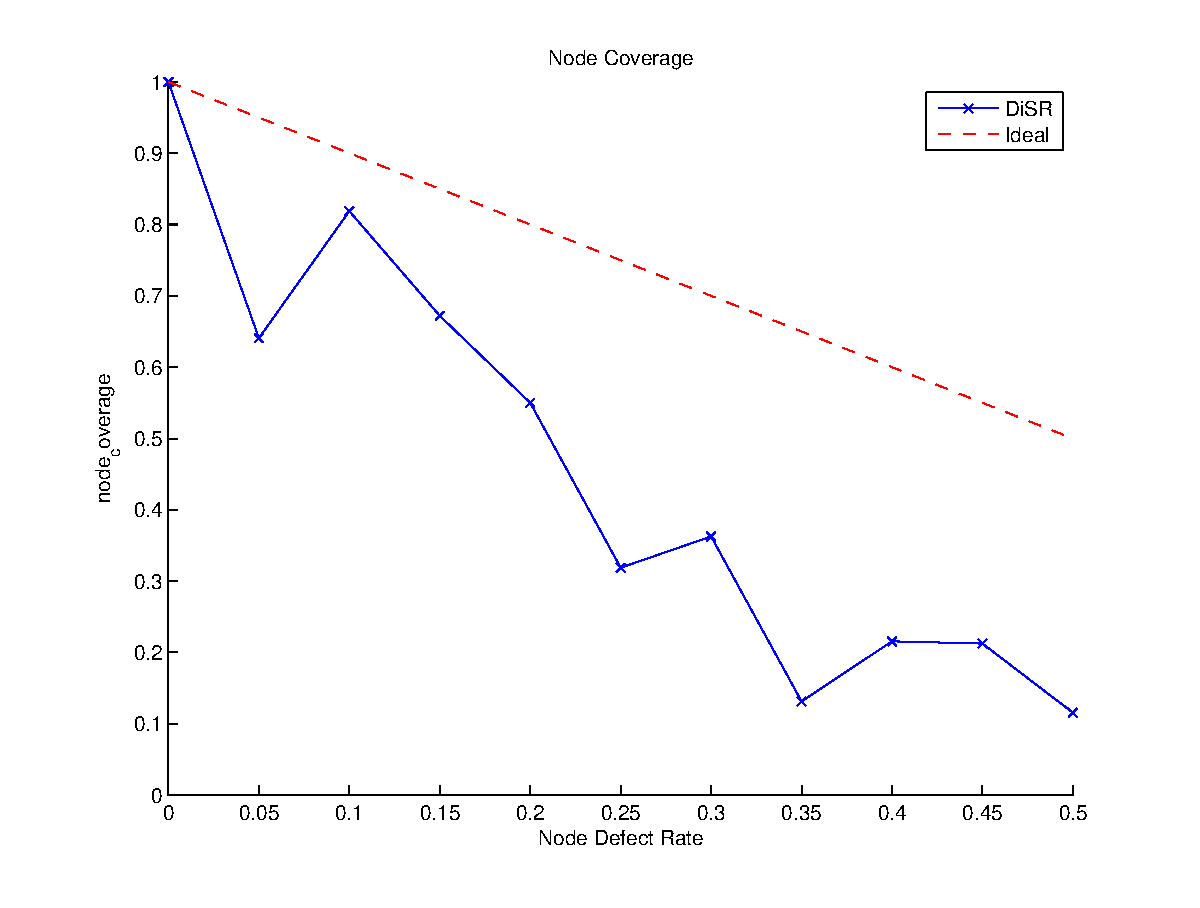
\includegraphics[width=0.23\textwidth]{pictures/set1.eps} & 
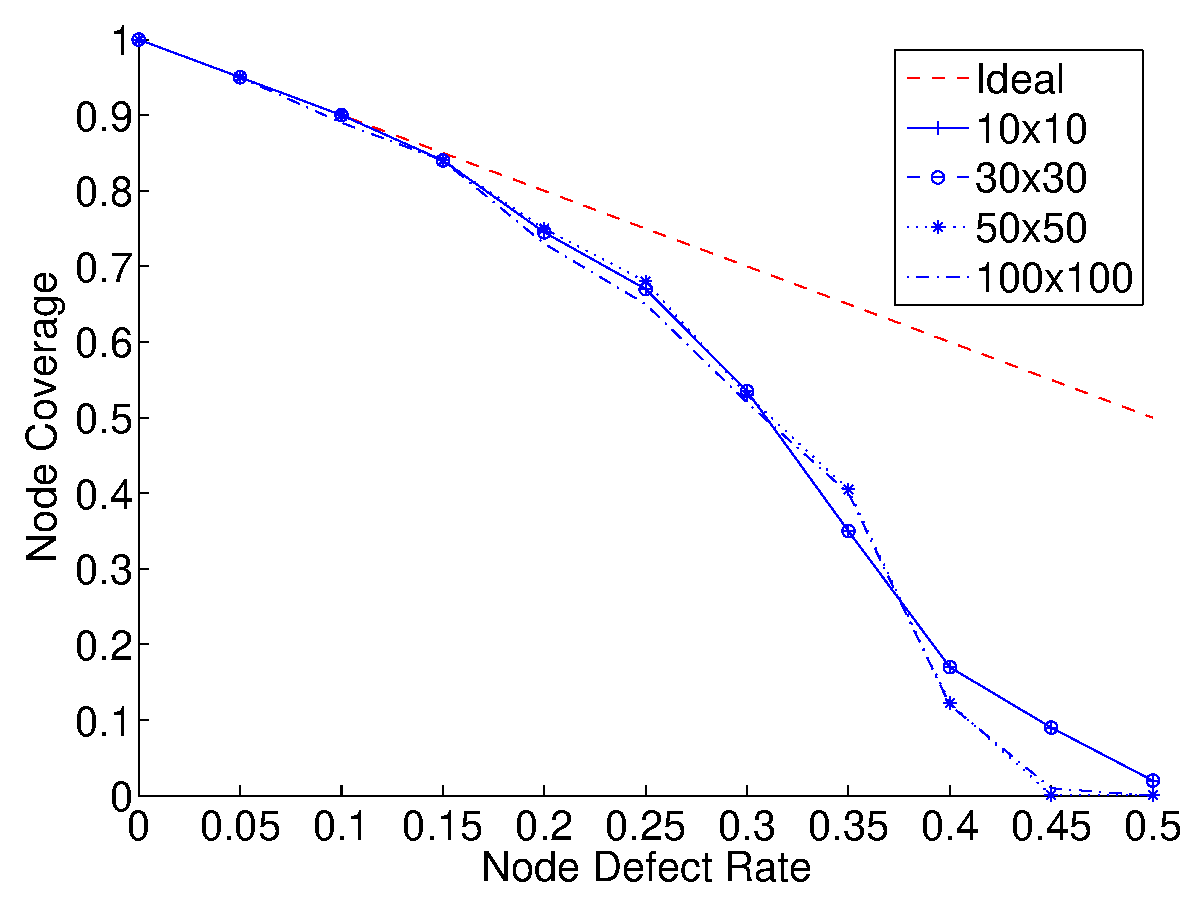
\includegraphics[width=0.23\textwidth]{pictures/coverage.eps} \\
(a) & (b) \\
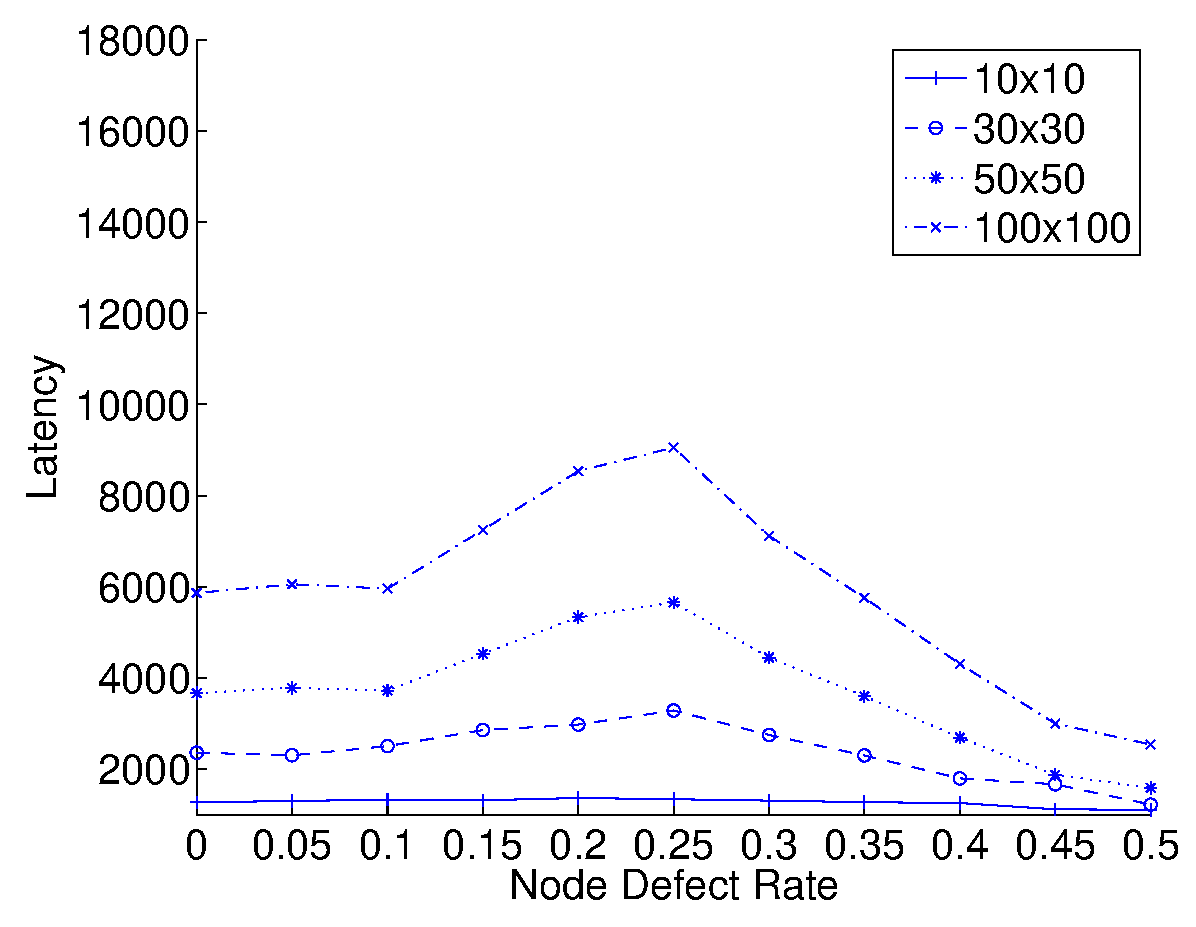
\includegraphics[width=0.23\textwidth]{pictures/set2.eps} & 
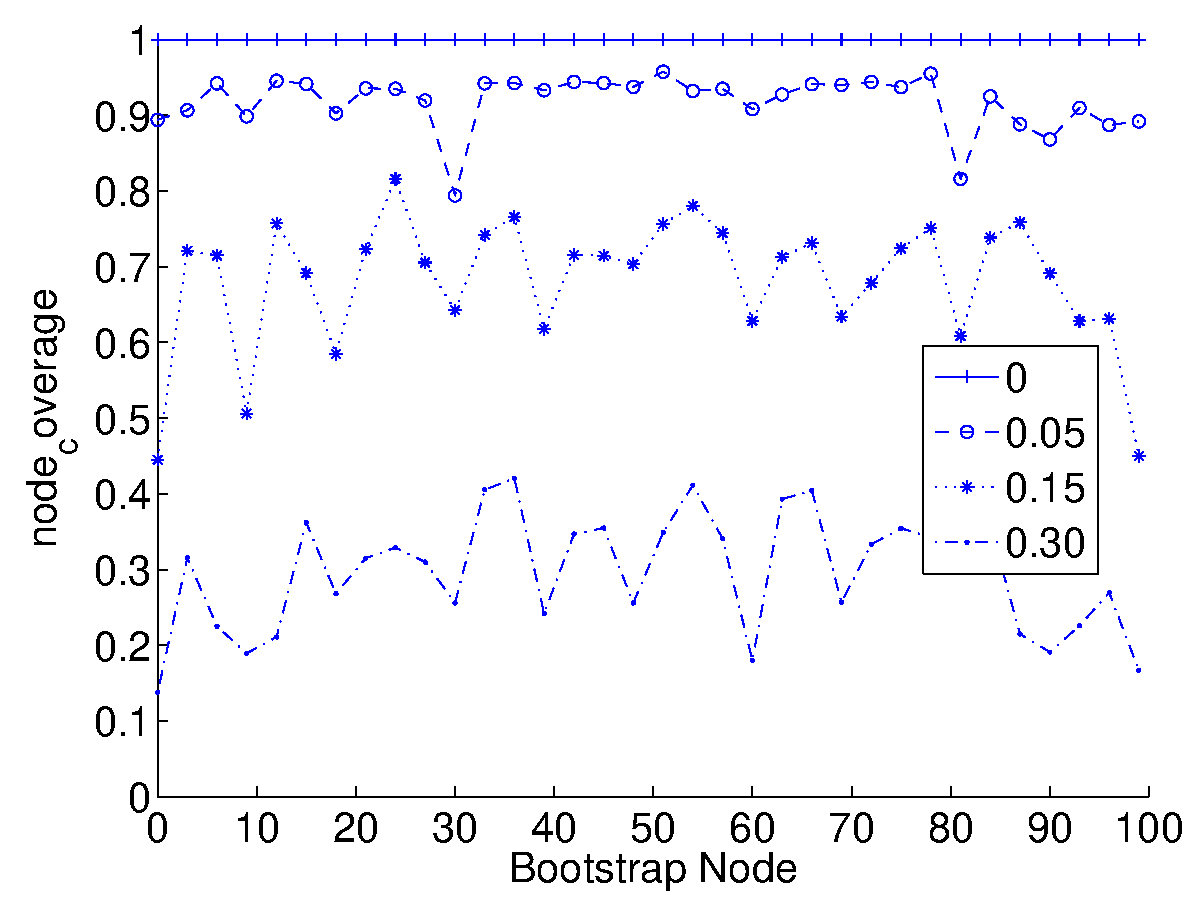
\includegraphics[width=0.23\textwidth]{pictures/set3.eps} \\
(c) & (d)
\end{tabular}
\caption{DiSR (a) and RPF (b) node coverage (c) Latency and effect
of bootstrap node (d)}
\label{fig:results}
\end{figure}

Finally, picture (d) visually represent  the stability of the approach
against different choices of the bootstrap node in a 10x10 network.
This is an important aspect to evaluate when considering that one of
the main advantages of DiSR against all the tree based approaches
should be the ability of choosing whatever bootstrap node, without
having to care of any particular \emph{root-node role} assumed in the future.
In other words, after segments have been established, the bootstrap node
is like every other node, i.e. it is not center of a structure, and it
is not an hotspot for the traffic distribution. The results in terms
of coverage,  shown for low, medium and high defect profiles, seems to
demonstrate a relatively limited impact of the bootstrap choice in
the low/medium scenarios, while a 30\%instability is found for very high defect
rates. This also sounds acceptable, since when lot of defective nodes
are present, the particular position of the bootstrap choice could
lead to completely different evolution in the DiSR setup process.


